\begin{figure}[htbp]
\centering
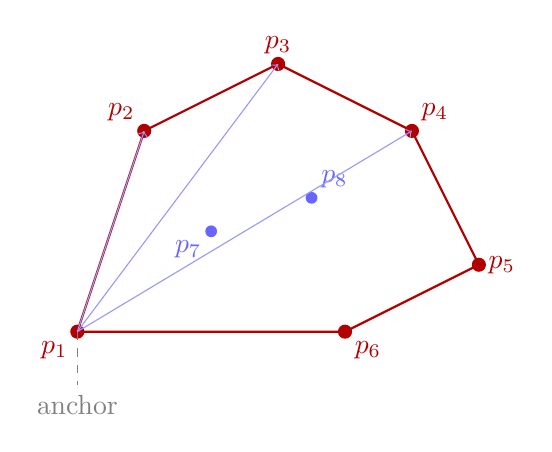
\begin{tikzpicture}[scale=0.85]
  \coordinate (p1) at (0,0);
  \coordinate (p2) at (1,3);
  \coordinate (p3) at (3,4);
  \coordinate (p4) at (5,3);
  \coordinate (p5) at (6,1);
  \coordinate (p6) at (4,0);
  \coordinate (p7) at (2,1.5);
  \coordinate (p8) at (3.5,2);
  \fill[blue!60] (p7) circle (2.5pt) node[below left] {$p_7$};
  \fill[blue!60] (p8) circle (2.5pt) node[above right] {$p_8$};
  \fill[red!70!black] (p1) circle (3pt) node[below left] {$p_1$};
  \fill[red!70!black] (p2) circle (3pt) node[above left] {$p_2$};
  \fill[red!70!black] (p3) circle (3pt) node[above] {$p_3$};
  \fill[red!70!black] (p4) circle (3pt) node[above right] {$p_4$};
  \fill[red!70!black] (p5) circle (3pt) node[right] {$p_5$};
  \fill[red!70!black] (p6) circle (3pt) node[below right] {$p_6$};
  \draw[thick,red!70!black] (p1)--(p2)--(p3)--(p4)--(p5)--(p6)--cycle;
  \draw[dashed,gray] (p1) -- ++(0,-0.8) node[below] {anchor};
  \draw[->,blue!40,thin] (p1) -- (p2);
  \draw[->,blue!40,thin] (p1) -- (p3);
  \draw[->,blue!40,thin] (p1) -- (p4);
\end{tikzpicture}
\caption{Graham Scan: the anchor point $p_1$ (lowest $y$) sorts all other points by polar angle. The hull vertices (red) are traced in counter-clockwise order.}
\label{fig:graham_scan}
\end{figure}
